\section{Network-On-Chip}

\sh{Evolution of Buses}
A network-on-chip is a communication system used in modern \acs{SoC} architectures to efficiently connect various components (e.g., processors, memory, and specialized units). Instead of using classic buses or point-to-point connections, \ac{NoC} relies on a network-like communication principle inspired by computer networks or high-performance computers \cite{serpanos_architecture_2011}.

Figure~\ref{fig:Evolution_of_Interconnection} shows the development of bus technologies over the past few years.
\begin{figure}[htbp]
    \centering
    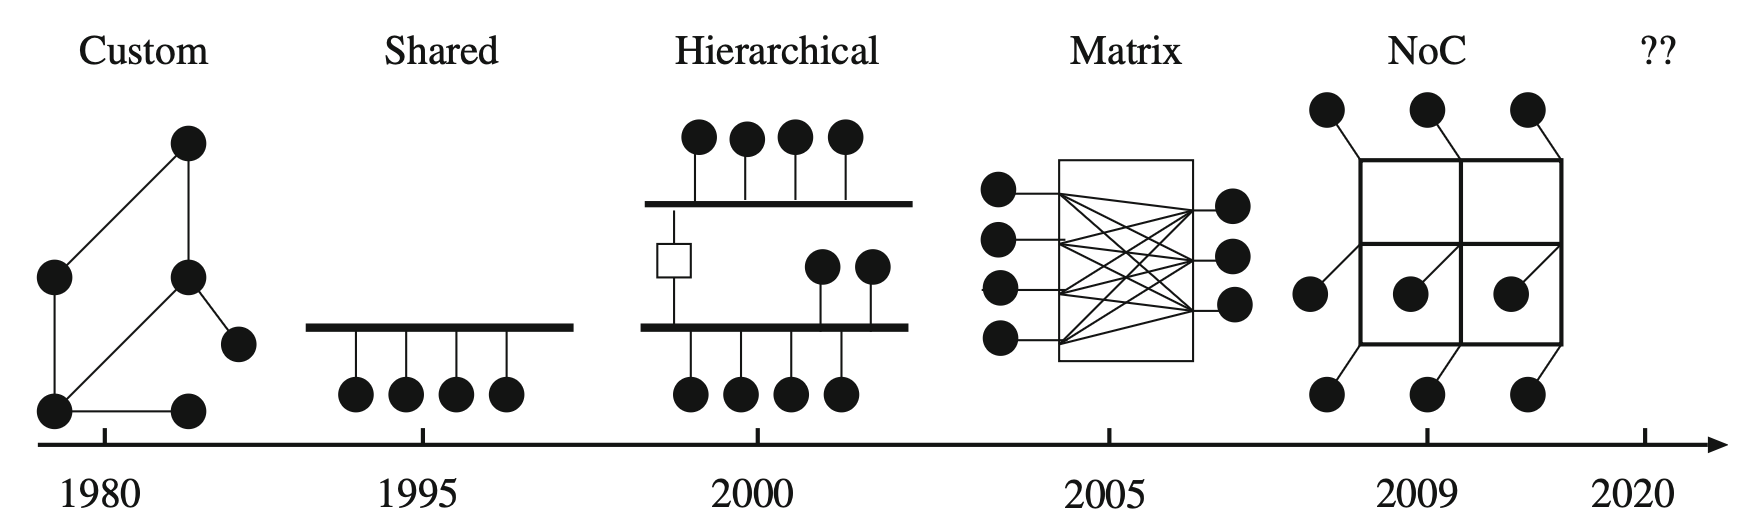
\includegraphics[width=0.95\textwidth]{img/Evolution of On-Chip communication interconnect.png}
    \caption{Evolution of Interconnections}
    \cite{abderazek_multicore_2013}
    \label{fig:Evolution_of_Interconnection}
\end{figure}

Before 1980, custom solutions were typically used for on-chip communication. Starting around 1995, so-called shared-bus architectures such as ARM’s AMBA bus~\cite{arm_amba_nodate} and IBM’s CoreConnect~\cite{international_business_machines_corporation_coreconnect_1999} were introduced. These approaches enabled a more modular design with standardized interfaces and supported the reuse of IP components (IP reuse)~\cite{unnikrishnan_network_2021}.

However, as bandwidth demands increased, shared-bus systems became a bottleneck. To address this issue, hierarchical bus architectures were introduced. These utilize multiple buses or bus segments to reduce the load on the main bus. Local communication between modules on the same bus segment is possible without burdening the entire bus. Nevertheless, such architectures are only limitedly scalable, inflexible, and lead to increased design complexity. The more cores are connected, the harder it becomes to meet timing constraints (time closure\footnote{Time Closure: Successfully ensuring all timing constraints are satisfied in the design so that the chip can operate reliably at its target clock frequency.}) and ensure \ac{QoS}~\cite{unnikrishnan_network_2021}.

Another alternative was the bus matrix — a full crossbar system that allows parallel connections between components. However, as system size grows, the complexity of wiring also increases and can eventually improve the effort required for the logic itself. Moreover, such systems do not clearly separate transport, transaction, and physical layers. Therefore, when a system upgrade is needed, it often affects the entire interface design and all connected blocks~\cite{unnikrishnan_network_2021}.

Against this background, some researchers in the early 2000s proposed implementing communication between different processing units on a chip via a predefined platform—an integrated switching network known as Network-on-Chip. \acp{NoC} fulfill key requirements of modern \ac{SoC}s: Reusability, scalable bandwidth, and energy efficiency. \acp{NoC} have replaced wired connections and instead utilize intelligent network infrastructures. They draw on models, techniques, and tools from network communication, thereby replacing fixed wiring with packet-based communication~\cite{unnikrishnan_network_2021}.

\begin{figure}[h!]
    \centering
    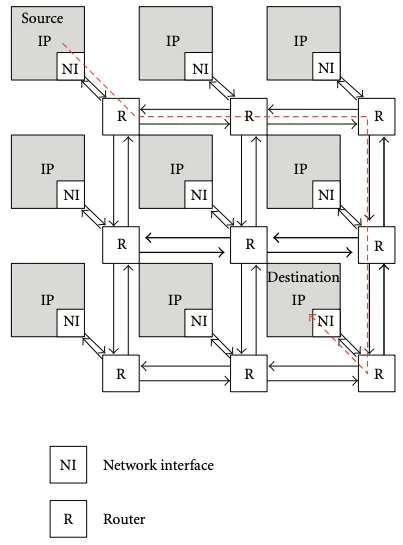
\includegraphics[width=0.5\textwidth]{paper/img/NoC-Components.png}
    \caption{NoC Components}
    \cite{hertz_why_2025}
    \label{fig:noc_components}
\end{figure}

\sh{NoC Components}
A \acs{NoC} consists - as you can see in figure~\ref{fig:noc_components} - of the following three essential components~\cite{yu_flexible_2010, unnikrishnan_network_2021}:

\begin{enumerate}
    \item \textbf{Links} physically connect routers and enable data transfer between them. A link may contain multiple logical channels, each implemented over a set of wires with synchronization logic.
    \item \textbf{Routers} establish the communication paths through switching matrices connecting multiple input and output ports. They implement routing and flow control policies that define the forwarding strategy.
    \item \textbf{\acp{NI}} bridge the IP cores and the NoC. Since IPs often communicate via bus protocols like AMBA~AXI, \acp{NI} translate transactions into packets suitable for the NoC.
\end{enumerate}

\iffalse
\sh{Topology}
The \ac{NoC} topology defines how routers are interconnected and is typically represented as a graph $G(N, C)$, where $N$ denotes routers and $C$ communication channels. 

Common \textit{direct topologies}, such as 2D meshes or tori, connect each router to neighboring nodes and one processing element. In \textit{indirect topologies}, some routers act solely as intermediate switches. The chosen topology strongly influences network latency, scalability, and implementation complexity~\cite{unnikrishnan_network_2021}.

\sh{Routing}
Routing determines how packets travel from source to destination. In \textit{deterministic routing}, such as XY or \ac{DOR}, the path is predefined and remains static. In contrast, \textit{adaptive routing} adjusts paths based on network conditions, enabling congestion avoidance and improved load balance~\cite{ma_summary_2024}.

Congestion-aware routing algorithms extend adaptive approaches by explicitly monitoring link utilization to distribute traffic more evenly and prevent bottlenecks~\cites{hu_dyad_2004}{fang_parrouting_2020}{luneque_routing_2013}.
\fi

\iffalse
\sh{Flow Control} 
Another essential aspect in \ac{NoC} systems is the so-called flow control, which defines how available resources such as bandwidth or buffer memory are assigned to individual data packets. The goal is to ensure efficient resource usage and thereby optimize the overall network throughput. Fundamentally, one distinguishes between bufferless and buffered flow control.

In \textit{bufferless flow control}, there are no or only very limited intermediate storage; data packets that cannot be forwarded immediately are either discarded or rerouted via alternative paths. A typical example is circuit switching, where a fixed path through the network is reserved prior to data transmission. In contrast, buffered flow control temporarily stores data packets when the desired output channel is occupied or forwarding is otherwise delayed. This method increases the flexibility of data transmission and reduces the likelihood of packet loss or rerouting, but entails higher hardware complexity and energy consumption due to the additional buffer resources that must be provided and managed. 

Within \textit{buffered flow control}, two central approaches can be distinguished: In packet-buffer flow control, the entire packet is stored in a buffer until it can be forwarded completely. This method is simple to implement but can be inefficient, especially for large packets and limited buffer memory. A finer control is provided by flit-buffer flow control, where packets are divided into smaller units called flits (flow control digits) and buffered individually. This allows more efficient use of available memory and better coordination of data flow, potentially leading to higher network performance. 

Additionally, different buffering strategies exist within these approaches, including \textit{input buffering}, \textit{output buffering}, and \textit{virtual channel buffering}. Input buffering stores incoming data streams at each input channel, while output buffering places buffers at the router’s output channels. Virtual channel buffering allows multiple logical channels to share one physical channel, thereby reducing blocking and improving the utilization of available bandwidth. However, this technique requires more complex control logic and increases hardware overhead.\cite{dally_principles_2004}
\fi

\iffalse
\sh{Protocol}
\begin{figure}[htbp]
    \centering
    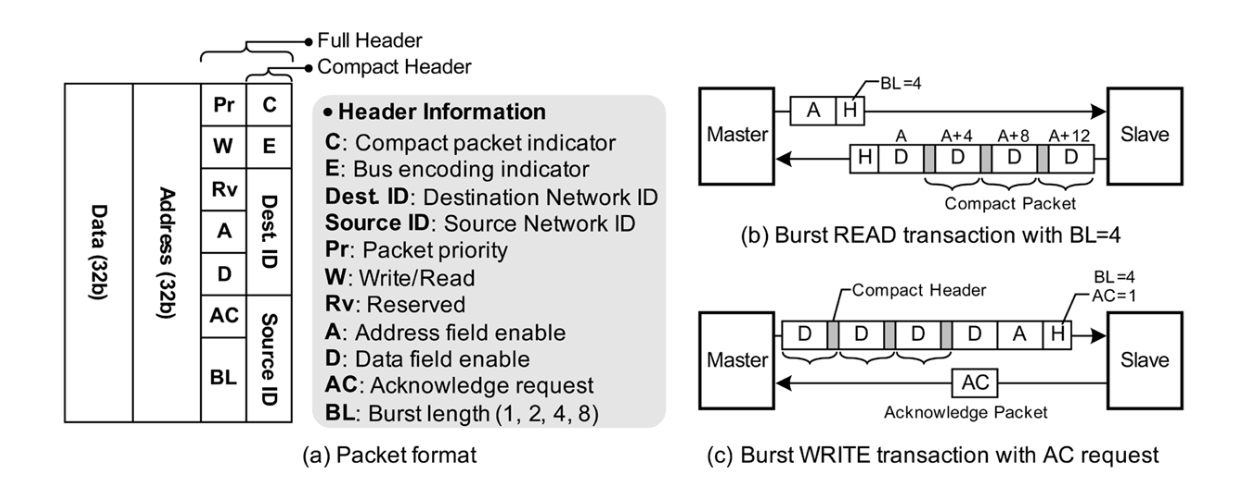
\includegraphics[width=0.95\textwidth]{img/NoC Protocol.png}
    \caption{NoC-Protocol~\cite{lee_low-power_2006}}\label{fig:NOC_Protocol}
\end{figure}

NoCs typically use packet-based communication protocols with flexible header fields containing routing, priority, and control information. This modularity allows efficient and scalable data exchange between components and supports the coexistence of different traffic classes~\cite{lee_low-power_2006}.

In many modern SoCs, bus-based transaction protocols such as AMBA~AXI serve as the interface between processing elements and the NoC. The network interface must therefore handle the translation between the transaction layer and the packet-based transport layer~\cite{lee_low-power_2006}.
\fi

\sh{Advantages and Disadvantages}
A \ac{NoC} offers several advantages over traditional bus-based communication structures: It enables scalable and parallel data transfer between many processor cores or components, significantly improving performance and efficiency in complex systems. Moreover, the structured interconnection enhances fault tolerance and bandwidth while reducing latency~\cite{dally_principles_2004}.

However, \acp{NoC} also bring disadvantages, such as increased design and implementation effort, as well as additional chip area and power consumption. In particular, the complexity of routing and control can complicate development and validation. Overall, however, in modern multicore systems the advantages of \acp{NoC} usually outweigh the disadvantages, as they provide a flexible and high-performance communication infrastructure~\cite{dally_principles_2004}.


\noindent\textit{Note:} 
Detailed discussions of NoC topology, routing, flow control, and protocol variations are omitted due to space limitations. 
For a detailed information about these subtopics, see~\cite{dally_principles_2004, unnikrishnan_network_2021, lee_low-power_2006, ma_summary_2024, hu_dyad_2004, fang_parrouting_2020, luneque_routing_2013}.
